\documentclass[12]{beamer}

\usepackage[russian]{babel}
\usepackage{tikz}

\usetheme[progressbar=frametitle]{metropolis}
\setbeamertemplate{frame numbering}[fraction]
\usefonttheme{metropolis}
\setbeamercolor{background canvas}{bg=white}


\title{Семинар 1}
\subtitle{Предпосылки квантовой механики. Равновесное тепловое излучение}
\author{}
\date{\today}
\institute {\large \textbf{Ключевые слова}: \\[6pt] Равновесное тепловое излучение, абсолютно черное тело, спектральная плотность излучения, формула Планка, закон смещения Вина, закон Стефана-Больцмана\\[6pt] \textbf{Задачи}: \\[6pt] 0-1-1, 0-1-2, 1.22, 1.23, 1.38}


\begin{document}
\metroset{block=fill}
\maketitle


\begin{frame}[t]{Проблемы классической физики}
\begin{itemize}
    \only<1->{\item \Large Модель атома Резерфорда}
    \only<3->{\item \Large Линейчатые спектры излучения и поглощения атомов}
    \only<5->{\item \Large Внешний фотоэффект}
    \only<7->{\item \Large Равновесное тепловое излечение}
\end{itemize}
\only<2>{
\begin{tikzpicture}[remember picture,overlay]
\node at (current page.center) {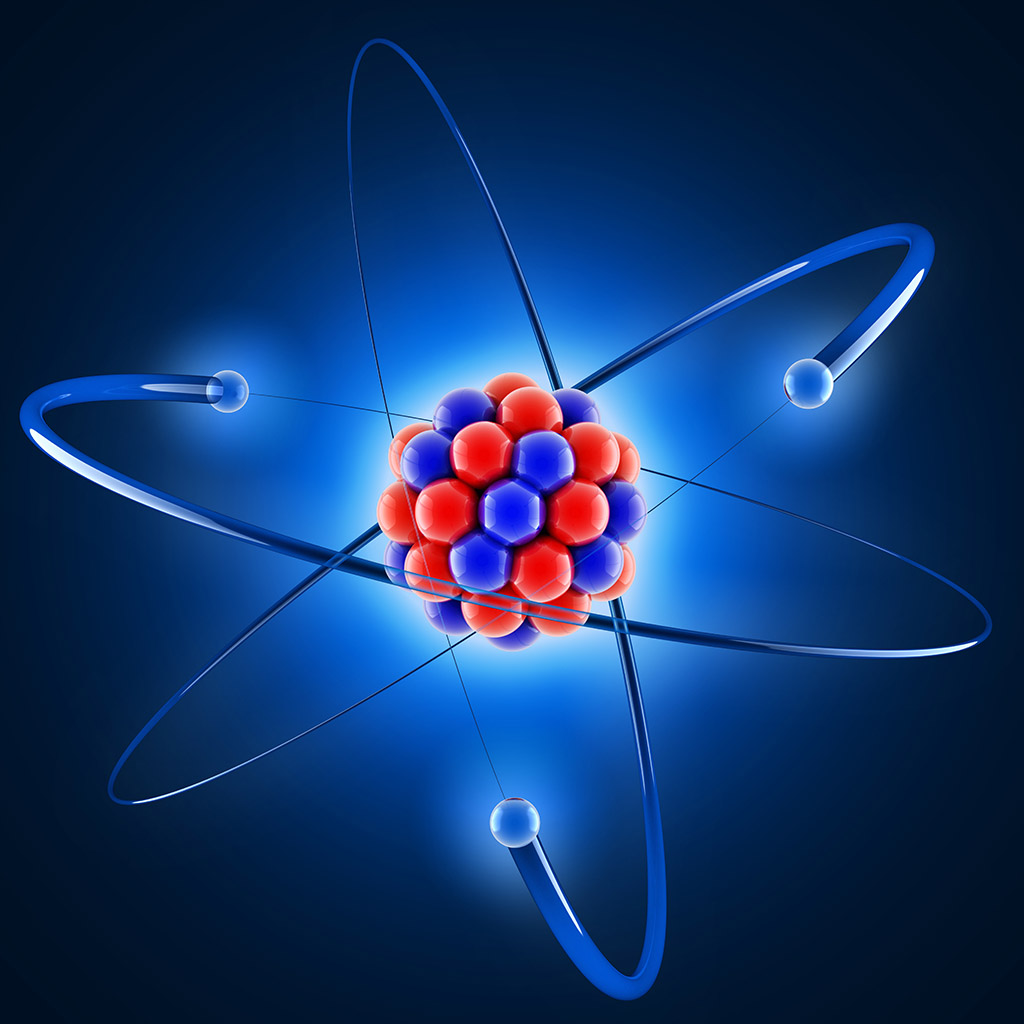
\includegraphics[height=0.9\textheight]{Seminar_01/pics/atom.jpg}};
\end{tikzpicture}}
\only<4>{
\begin{tikzpicture}[remember picture,overlay]
\node at (current page.center) {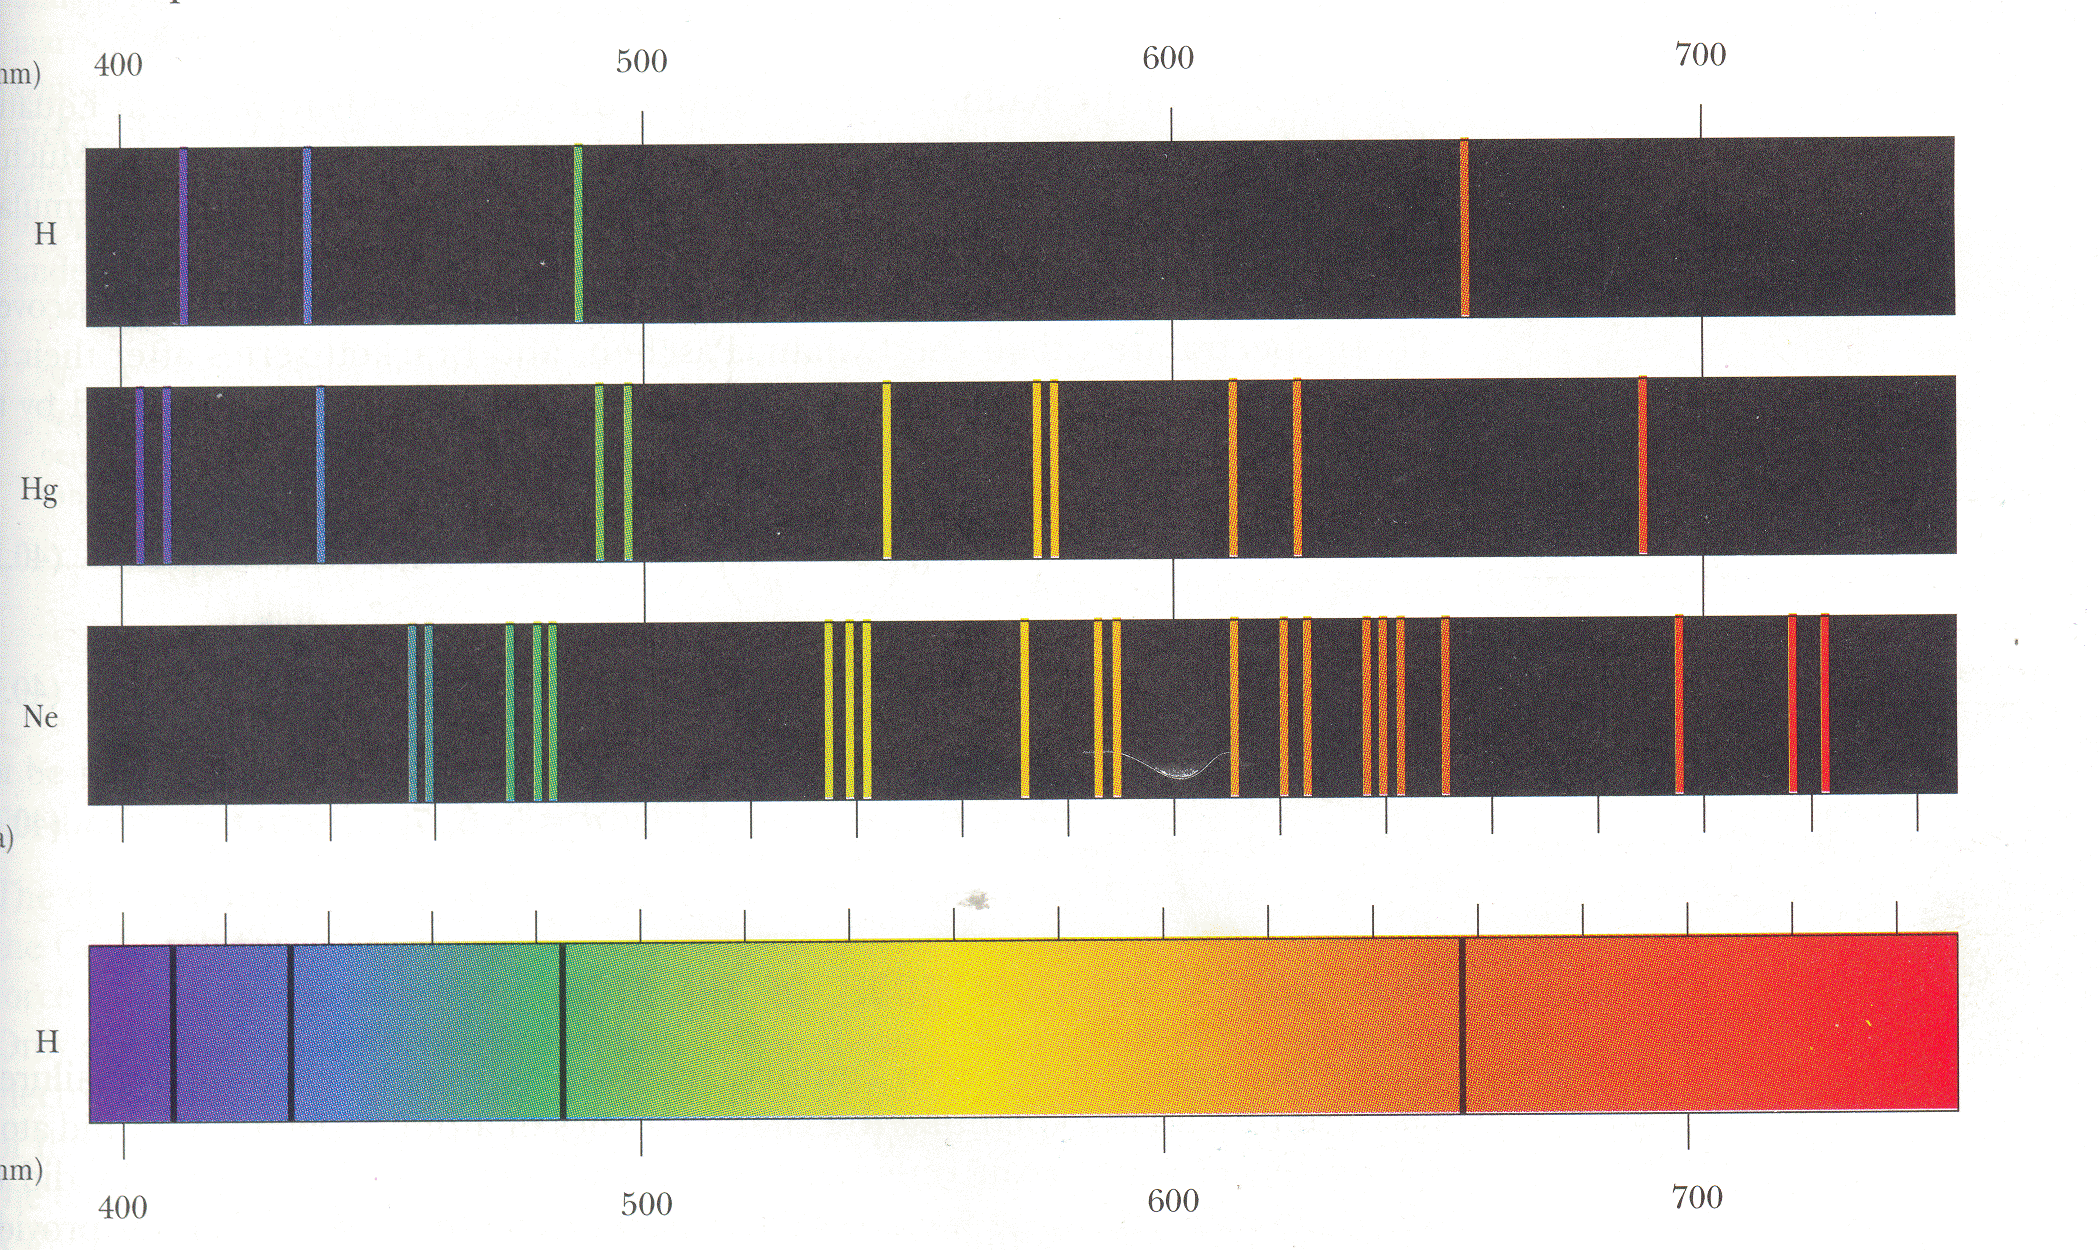
\includegraphics[height=0.8\textheight]{Seminar_01/pics/atom_specter.png}};
\end{tikzpicture}}
\only<6>{
\begin{tikzpicture}[remember picture,overlay]
\node at (current page.center) {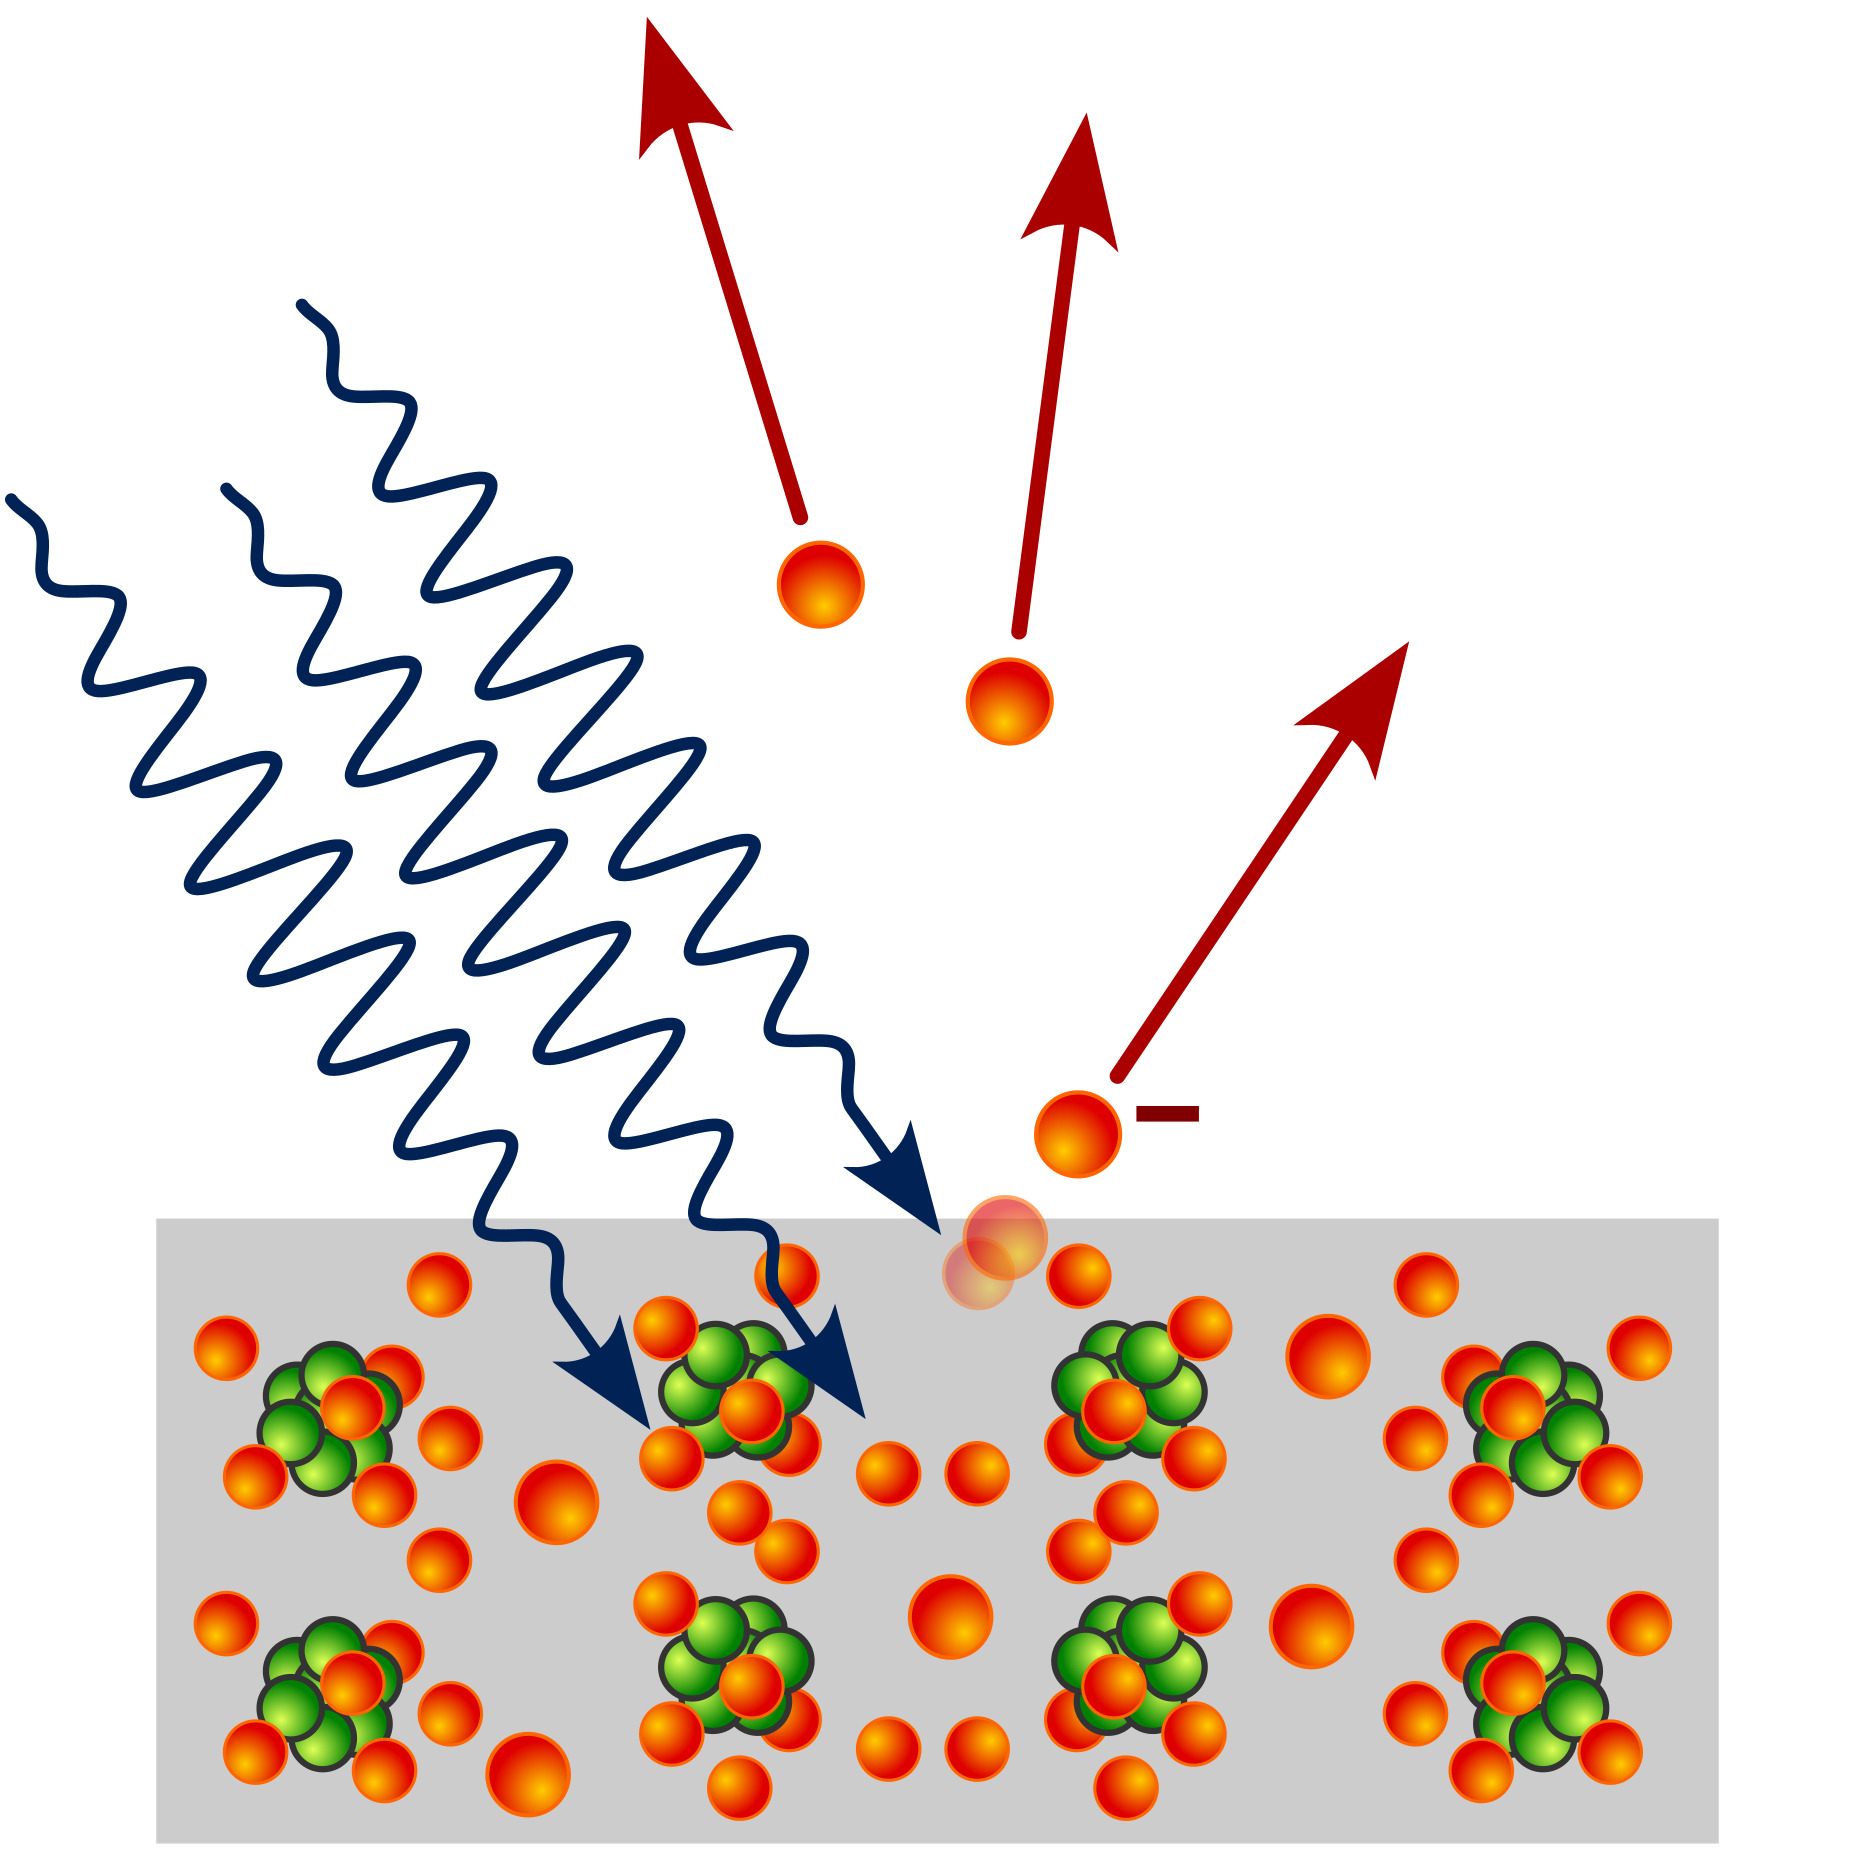
\includegraphics[height=0.8\textheight]{Seminar_01/pics/photoelectric_effect.jpg}};
\end{tikzpicture}}
\end{frame}

\begin{frame}[t]{Равновесное тепловое излучение}
\begin{block}{Тепловое излучение}
Электромагнитное излучение, испускаемое телами за счёт их внутренней энергии. 
\end{block}
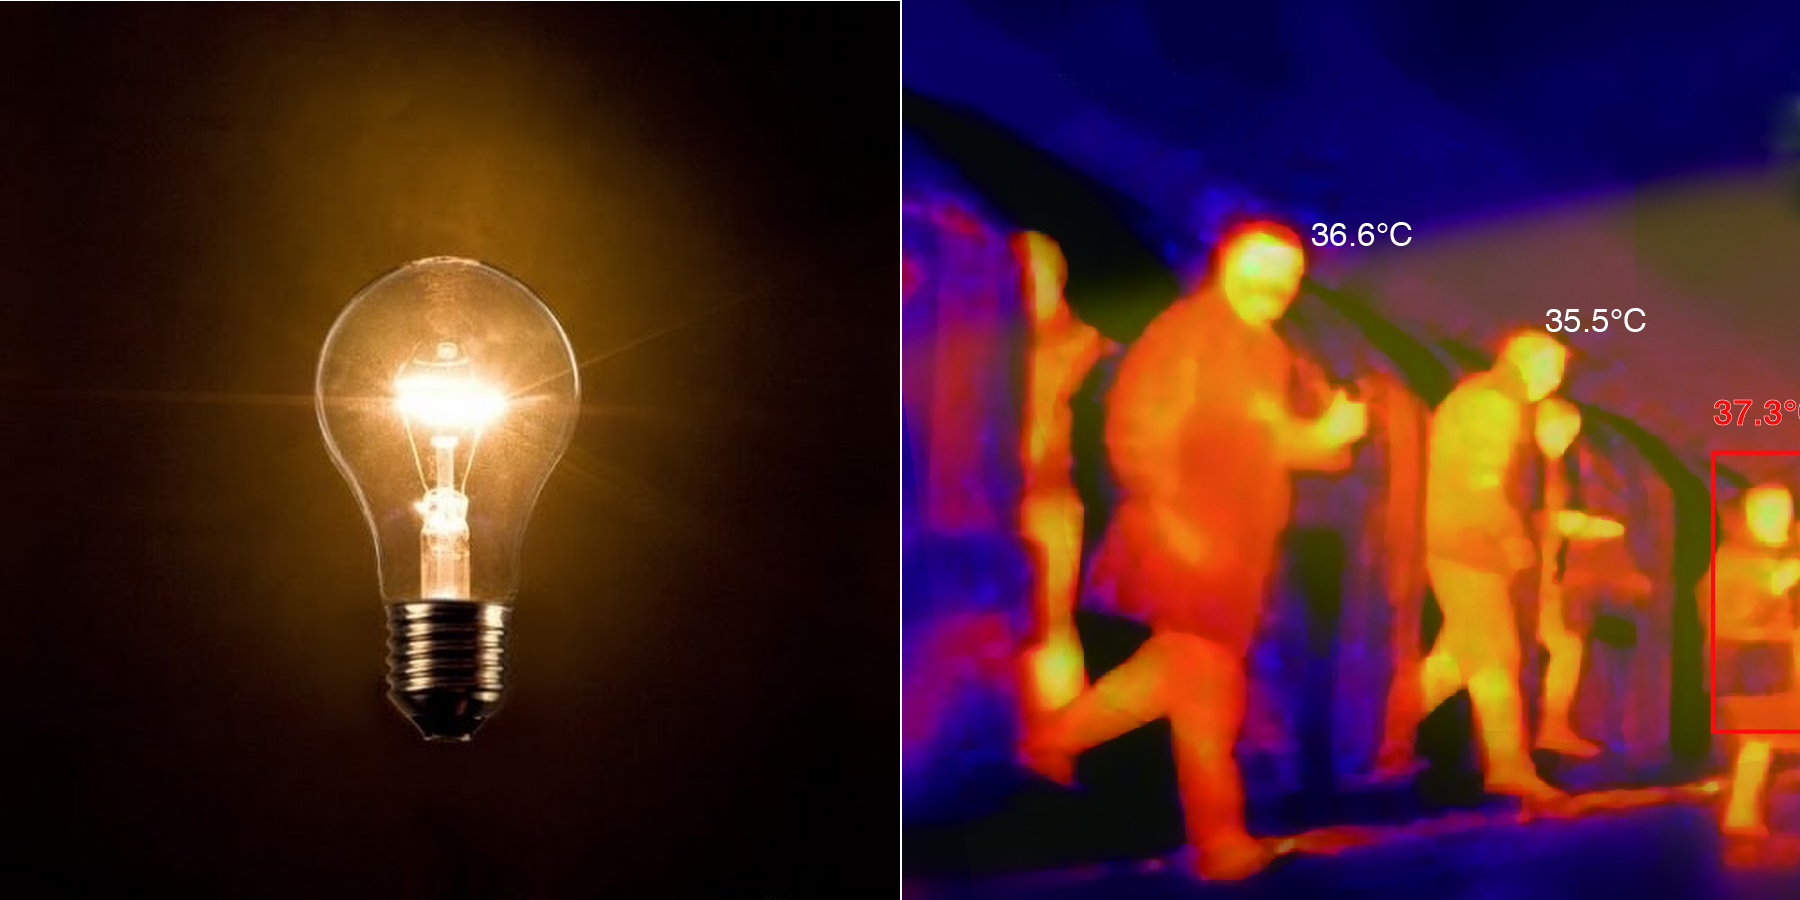
\includegraphics[width=\textwidth]{Seminar_01/pics/pic_01.png}
\end{frame}

\begin{frame}[t]{Модель абсолютно черного тела}
\begin{block}{Абсолютно черное тело, АЧТ}
Тело, которое поглощает всё падающее излучение и равновесным образом переизлучает его 
\end{block}
\only<2->{
\begin{columns}[onlytextwidth]
\column{0.6\textwidth}
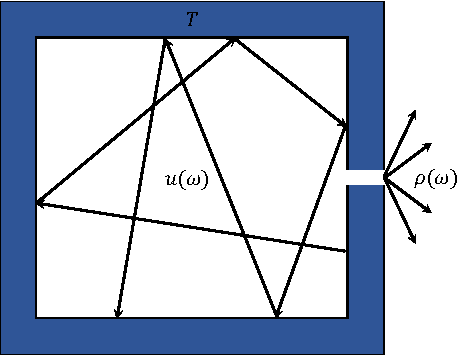
\includegraphics[width=\textwidth]{Seminar_01/pics/pic_02.pdf}
\column{0.4\textwidth}
\begin{itemize}
    \item[] $u(\omega) = \dfrac{dE}{d\omega}$  плотность энергии излучения
    \item[] $\rho(\omega) = \dfrac{dE/d\omega}{dSdt}$  спектральная плотность изучения
    \only<3>{\item[] $\rho(\omega) = \dfrac{cu(\omega)}{4}$}
\end{itemize}
\end{columns}}
\end{frame}

\begin{frame}[t]{Резонатор как классическая модель излучения}\scriptsize
\begin{block}{Разрешенные моды в резонаторе}
$$ k_x = \dfrac{\pi A}{L}, k_y = \dfrac{\pi B}{L}, k_z = \dfrac{\pi C}{L}; A, B, C\in \mathbb{N}$$
\end{block}
\only<2->{
\begin{columns}[onlytextwidth]
\column{0.5\textwidth}
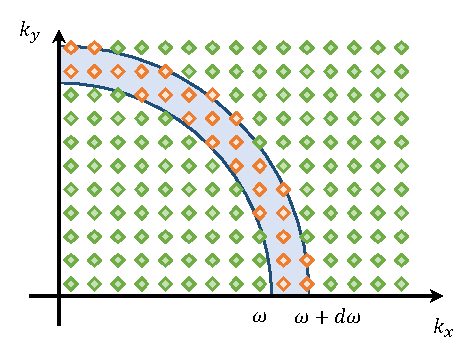
\includegraphics[width=\textwidth]{Seminar_01/pics/pic_03.pdf}
\column{0.5\textwidth}
\begin{block}{Расчет плотности разрешенных состояний}
Поверхность постоянной частоты -- сфера, т.к. \omega^2 = k^2c^2\\
Тогда плотность состояний:
$$dN  \sim \omega^2d\omega \Rightarrow \dfrac{dN}{d\omega} \sim \omega^2$$
\end{block}
\end{columns}}
\only<3->{
\begin{alertblock}{Ультрафиолетовая катастрофа}
$$E = \int\limits_{0}^{+\infty} 2kT\dfrac{dN}{d\omega}d\omega \rightarrow \infty$$
\end{alertblock}
}
\end{frame}

\begin{frame}[t]{Формула планка}\scriptsize
\begin{block}{Гипотеза Планка}
На данной частоте может быть запасено только целое число квантов колебаний $E_n =n \hbar \omega$
$$\langle E \rangle = \dfrac{\sum\limits_{n=0}^{\infty} E_n \exp{\left(-\dfrac{\hbar \omega}{kT}\right)}}{\sum\limits_{n=0}^{\infty} \exp{\left(-\dfrac{\hbar \omega}{kT}\right)}} = \dfrac{\hbar \omega}{\exp{\left(\dfrac{\hbar \omega}{kT}\right)} - 1}$$
\end{block}
\only<2->{
\begin{block}{Формула Планка}
\begin{gather*}
    \rho(\omega)d\omega = \dfrac{\hbar \omega^3}{4\pi^2c^2\left[ \exp{\left(\dfrac{\hbar \omega}{kT}\right)} - 1\right]}d\omega\\
    \rho(\lambda) d\lambda = \dfrac{\pi h c^2}{\lambda^5\left[ \exp{\left(\dfrac{\hbar c}{\lambda kT}\right)} - 1\right]}d\lambda
\end{gather*}
\end{block}
}
\end{frame}

\begin{frame}[t]{Закон смещения Вина. Закон Стефана-Больцмана}\scriptsize
\textbf{Графики спектральной плотности излучения}
\begin{columns}[onlytextwidth]
\column{0.5\textwidth}
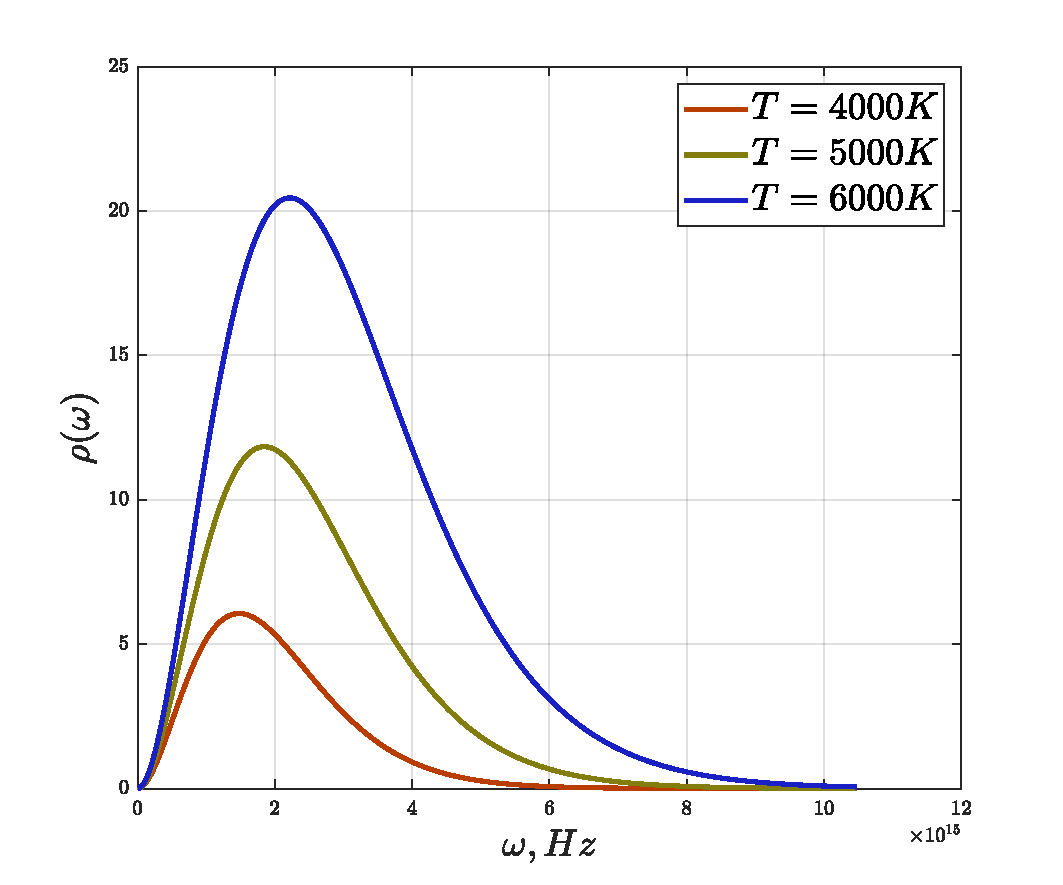
\includegraphics[width=\textwidth]{Seminar_01/pics/pic_04_left.pdf}
\column{0.5\textwidth}
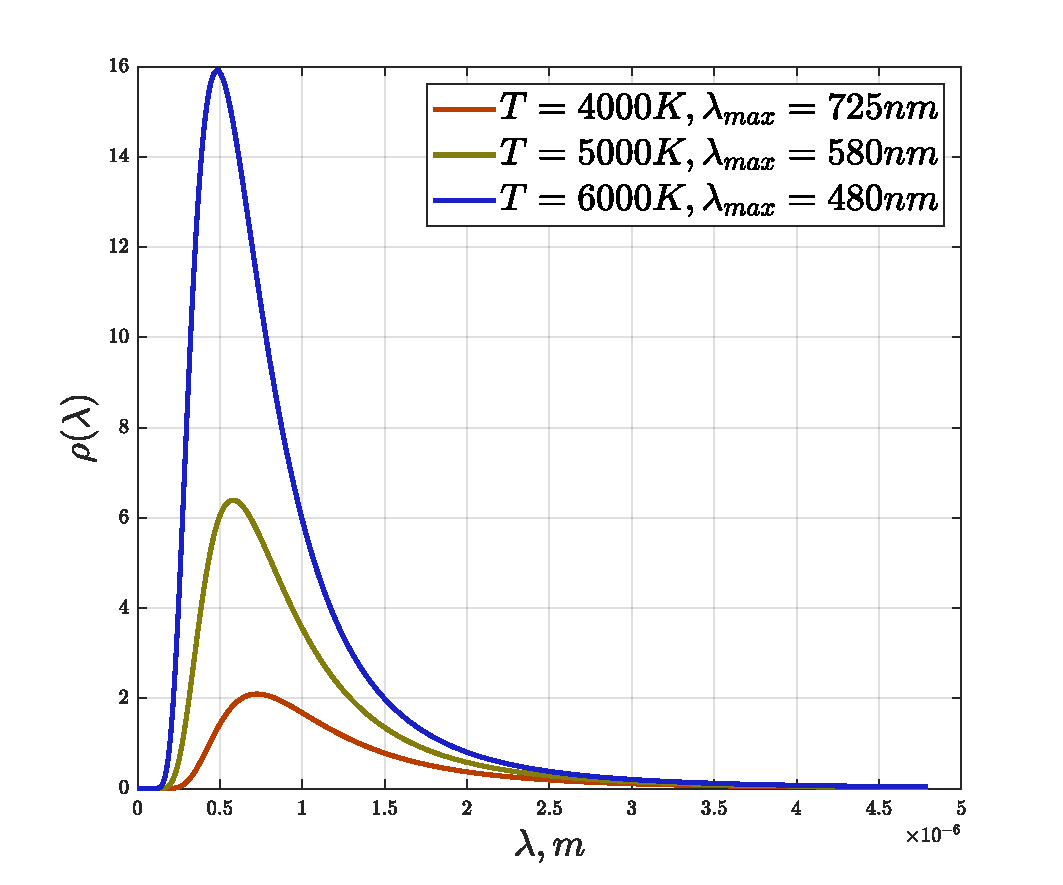
\includegraphics[width=\textwidth]{Seminar_01/pics/pic_04_right.pdf}
\end{columns}
\only<2->{
\begin{columns}[t, onlytextwidth]
\column{0.59\textwidth}
\begin{block}{Закон Стефана-Больцмана}
\begin{equation*}
\label{eq:sem_01_stefan_boltzman}
    P_{total} = \int\limits_{0}^{\infty}\dfrac{\hbar \omega^3}{4\pi^2c^2\left[ \exp{\left(\dfrac{\hbar \omega}{kT}\right)} - 1\right]}d\omega = \sigma T^4
\end{equation*}
\end{block}
\column{0.4\textwidth}
\begin{block}{Закон  Вина}
\begin{equation*}
    \lambda_{max} = \dfrac{2.9 \cdot 10^6}{T \text{[K]}} \text{ нм}
\end{equation*}
\end{block}
\end{columns}}
\end{frame}

\begin{frame}{Задачи 0-1-1, 0-1-2}\scriptsize
\begin{block}{Задача 0-1-1}
Вследствие повышения температуры положение максимума спектральной  энергетической  светимости  абсолютно  черного  тела  переместилось  с  2 мкм на 1 мкм. Во сколько раз изменилась его интегральная энергетическая светимость?
\\[10pt]
\begin{equation*}
    \dfrac{T}{T_0} = \dfrac{\lambda_0}{\lambda} \Rightarrow \dfrac{P}{P_0} = \dfrac{T^4}{T^4_0} = \dfrac{\lambda^4_0}{\lambda^4} = 2^4 =16 
\end{equation*}
\end{block}

\begin{block}{Задача 0-1-2}
Оценить давление теплового излучения во внутренней области Солнца, где температура равна $1.3\cdot 10^7$ К?\\[10pt]
\begin{equation*}
    p=\int\limits_0^{+\infty}\dfrac{1}{3}u(\omega) = \int\limits_0^{+\infty}\dfrac{4}{3}c\rho(\omega) = \dfrac{4}{3}c\sigma T^4 = 6.5\cdot 10^{29} \text{ Па}
\end{equation*}
\end{block}
    
\end{frame}

\begin{frame}{Задачи 1.22}\scriptsize
\begin{block}{Условие}
Спектр излучения космического рентгеновского источника соответствует спектру АЧТ. Максимум плотности излучения соответствует $\lambda_{max} = 2$ \AA, а суммарная по спектру плотность потока на Земле равна $j = 10^{-11} \text{ Вт}/\text{см}^2$. Расстояние от источника до Земли $L = 1.3\cdot 10^4$ световых лет. Оценить диаметр источника. 
\end{block}
\begin{block}{Решение}
\begin{gather*}
    \sigma T^4 \cdot 4\pi\left( \dfrac{D}{2}\right)^2 = j\cdot4\pi L^2 \\
    T = \dfrac{0.29 \text{ \AA}}{\lambda_{max}} \approx 1.5 \cdot 10^7 K
\end{gather*}
Окончательно $D\approx15.5$ км
\end{block}
    
\end{frame}

\begin{frame}{Задачи 1.23}\scriptsize
\begin{block}{Условие}
АЧТ подвешено в вакуумной установке так, что через оптическое окно на него падает солнечный свет. Если стенки установки охладить до температуры $T_{\text{ст1}} = 77 $ К, то тело будет иметь температуру $T_{1} = 275 $ К. Какова будет температура тела $T_2$, если $T_{\text{ст2}} = 295 $ К.
\end{block}
\begin{block}{Решение}
$\Phi$ -- поток излучения от Солнца 
\begin{gather*}
    S_{\text{тела}}\sigma T^4_{\text{ст1}} + \Phi = S_{\text{тела}}\sigma T^4_1\\
    S_{\text{тела}}\sigma T^4_{\text{ст2}} + \Phi = S_{\text{тела}}\sigma T^4_2\\
\end{gather*}
Вычтем из одного из уравнений другое и получим выражение для $T_2$:
\begin{equation*}
    T_2^4 = T_1^4 + T^4_{\text{ст2}} - T^4_{\text{ст1}} = 340 K
\end{equation*}
\end{block}
    
\end{frame}

\begin{frame}{Задачи 1.38}\scriptsize
\begin{block}{Условие}
Напряжение в сети возросло на 5 \%. На сколько процентов увеличится освещенность, создаваемая вакуумной лампой накаливания с температурой нити $T = 1500$ К на длине волны 500 нм. Нить можно считать абсолютно черны телом, рассмотреть случай когда $R(T) = const$ и $R(T) = R_0 + \alpha (T - T_0)$
\end{block}
\begin{block}{Решение}
Сравним $hc/\lambda \sim 10^{-19}$ и $kT\sim10^{-21}$, чтобы не тянуть за собой всю формулу Планка.
\begin{equation*}
    \rho(\lambda) \sim \exp{\left(-\dfrac{hc}{\lambda kT} \right)} \Rightarrow \ln{\rho(\lambda)} = -\dfrac{hc}{\lambda kT} \Rightarrow \dfrac{\Delta \rho}{\rho} = \dfrac{hc}{\lambda kT} \cdot \dfrac{\Delta T}{T}
\end{equation*}
Теперь учтем что вся мощность переходит в излучение: $\dfrac{V^2}{R} \propto T^4$
\begin{gather*}
    \text{Случай } R(T) = const \Rightarrow V^2 \propto T^4 \Rightarrow 2\dfrac{\Delta V}{V} = 4\dfrac{\Delta T}{T}\\
    \text{Случай } R(T) \propto T \Rightarrow V^2 \propto T^5 \Rightarrow 2\dfrac{\Delta V}{V} = 5\dfrac{\Delta T}{T}
\end{gather*}
\end{block}
\end{frame}

\begin{frame}[t]{Комментарии к задачам из задания}\scriptsize
\begin{itemize}
    \item Задача 1.22 Решена
\item Задача 1.26 Землю здесь вполне спокойно можно считать АЧТ и просто записать баланс энергий -- сколько пришло от Солнца (попало на Землю) и сколько излучилось с поверхности Земли
\item Задача 1.30 Закон Стефана-Больцмана в явном виде
\item Задача 1.38 Решена
\item Задача 1.44 Вывод закона Стефана-Больцмана, но не для всех частот, а только для некоторых. Интеграл, который там получится можно взять численно в вольфраме или забить и оценить его.
\item Задача 1.50 Решена в задачнике плюс отсылки на прошлый семестр. Посмотрим как кто помнит оптику
\end{itemize}
\end{frame}

\end{document}